\documentclass{article}
\usepackage{titling}
\usepackage[absolute]{textpos}
\setlength{\TPHorizModule}{10mm}
\setlength{\TPVertModule}{10mm}
\usepackage[top=2.5cm, bottom=2.5cm, left=3cm, right=2.5cm]{geometry}
\usepackage[polish]{babel}
\usepackage{polski}
\usepackage[utf8]{inputenc}
\usepackage{graphicx}
\usepackage{floatrow}
\linespread{1.5}
\title{Narzędzie wspomagające tworzenie ciągów przetwarzania wideo w oparciu o bibliotekę GStreamer}
\author{Marcin Kolny}
\usepackage[T1]{fontenc}
\usepackage{helvet}
\renewcommand*{\familydefault}{\sfdefault}
\renewcommand{\maketitle}{
  \begin{titlepage}
    \begin{figure}  
      
\includegraphics[width=40mm]{img/polsl-logo.png}
    \end{figure}
    \begin{center}
      \begingroup
      \fontsize{18pt}{21pt}\selectfont
      \textbf{Politechnika Śląska\\
        Wydział Automatyki, Elektroniki i Informatyki\\
        Kierunek Informatyka}\\
      \vspace{22mm}
      Projekt inżynierski\\
      \vspace{22mm}
      \endgroup
      \begingroup
      \fontsize{14pt}{17pt}\selectfont
      \thetitle \\
      \endgroup
      \vspace{30mm}
    \end{center}
    \begin{textblock}{14}(2.5,21.5)
      \fontsize{14pt}{17pt}\selectfont
      Autor: \theauthor \\
      Kierujący pracą: dr Ewa Lach\\
    \end{textblock}
    \begin{textblock}{20}(2.5,26.5)
      \fontsize{14pt}{17pt}\selectfont
      Gliwice, styczeń 2014\\
    \end{textblock}

  \end{titlepage}
}

\begin{document}
\maketitle
\tableofcontents
\cleardoublepage
\section{Biblioteka GStreamer}
\subsection{Opis biblioteki GStreamer}
\paragraph{}
Biblioteka GStreamer służy do konstruowania grafów przetwarzania strumieni multimedialnych. Biblioteka została napisana w języku ANSI C, i dostępna jest pod systemami Linux, Windows, OS X oraz Android.
\paragraph{}
GStreamer wydany jest na licencji GNU GPL, i może być wykorzystywany w zastosowaniach komercyjnych. Licencja pozwala również na modyfikowanie i dystrybucję kodu źródłowego biblioteki.
Biblioteka oferuje użytkownikowi wiele dostępnych już elementów do przetwarzania wideo(np. enkodery czy dekodery audio-video), do generowania sygnałów multimedialnych, a także do prezentacji wyników użytkownikowi. Ponadto, istnieje możliwość pisania własnych elementów, których można następnie użyć w bilbliotece GStreamer.
\subsection{Model programu}
\subsubsection{Elementy (ang. \textit{elements})}
\paragraph{}
Model programu biblioteki GStreamer oparty jest o elementy. Elementem nazywany jest obiekt, który realizuje zadany algorytm. Przykładowym elementem jest dekoder, którego celem jest dekodowanie strumienia multimedialnego o zadanym formacie.
\paragraph{}
Element może zawierać gniazda, dzięki którym możliwe jest połączenie go z innymi elementami(tzw. \textit{pad}).\\ 
Elementy, zawierające tylko gniazda wejściowe, nazywane są \textit{sink elements}, natomiast elementy posiadające tylko gniazda wejściowe, to tzw. \textit{source elements}. Elementy zawierające zarówno gniazda wejściowe, jak i wyjściowe, to \textit{filter elements}.
\begin{figure}[H]
  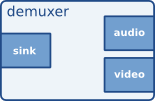
\includegraphics[width=40mm]{img/sample-demuxer.png}
  \caption{Przykładowy element typu \textit{demuxer}}
  \label{fig:sampleDemuxer}
\end{figure}
\paragraph{}
Na rysunku ~\ref{fig:sampleDemuxer} pokazany jest element \textit{filter element}, zawierający dwa gniazda wyjściowe, i jedno gniazdo wejściowe(jest to szczególny wariant filtra, tzw. \textit{demuxer}).
\subsubsection{Kontenery (ang. \textit{bins})}
\paragraph{}
Kontener jest szczególnym elementem. Podobnie, jak elementy, kontenery posiadają gniazda. Natomiast algorytmy zdefiniowane w elemencie-kontenerze realizowane są poprzez inne elementy, które agregowane są w danym kontenerze. Rysunek ~\ref{fig:sampleBin} przedstawia przykładowy kontener, zawierający dwa elementy, oraz jedno gniazdo wejściowe.
\begin{figure}[H]
  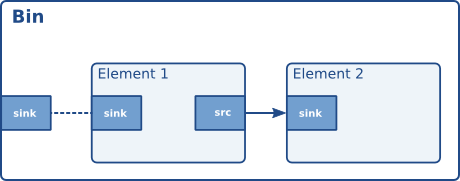
\includegraphics[width=100mm]{img/sample-bin.png}
  \caption{Przykładowy kontener}.
  \label{fig:sampleBin}
\end{figure}
\subsubsection{\textit{Pipeline}}
\paragraph{}
\textit{Pipeline} jest klasą pochodną obiektu \textit{bin}(a co za tym idzie, \textit{pipeline} jest również pochodną elementu). Jest to kontener nadrzędny całego modelu programu. Przechowuje w sobie najbardziej zewnętrzne elementy. \textit{Pipeline} nie posiada żadnych gniazd. Na rysunku ~\ref{fig:samplePipeline} pokazany został przykładowy \textit{pipeline}, realizujący operację odtwarzania strumienia audio-video z pliku ogg.
\begin{figure}[H]
  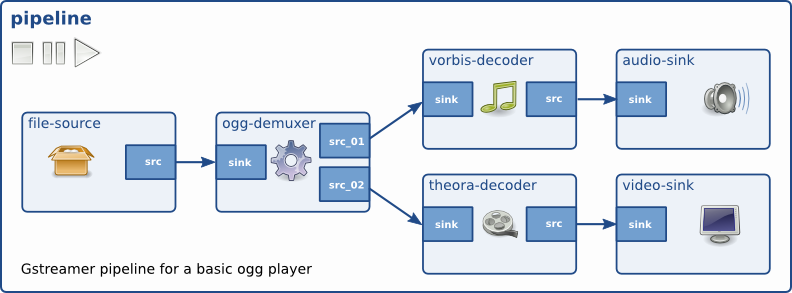
\includegraphics[width=150mm]{img/simple-player.png}
  \caption{Przykładowy \textit{pipeline}}
  \label{fig:samplePipeline}
\end{figure}
\subsubsection{Gniazda (ang. \textit{pads})}
\paragraph{}
Gniazda to obiekty umożliwiające połączenie ze sobą dwóch różnych elementów. Gniazdo charakteryzuje się dwoma właściwościami: kierunkiem oraz dostępnością. Pod względem kierunku, gniazda podzielone są na dwie grupy:
\begin{enumerate}
  \item wejściowe, tzw. \textit{sink pads},
  \item wyjściowe, tzw. \textit{src pads}.
\end{enumerate}
\paragraph{}
Gniazda wyjściowe(inaczej, źródłowe), służą do przesyłania danych do następnego elementu. Gniazda wejściowe wykorzystywane są natomiast do odbierania danych przesłanych z poprzednich elementów.
\paragraph{}
Kolejna właściwość, dzieli zbiór gniazd na trzy grupy:
\begin{enumerate}
  \item występujące zawsze(\textit{always pads}),
  \item występujące w zależności od danych(\textit{sometimes pads, dynamic pads}),
  \item pojawiające się na żądanie użytkownika(\textit{request pads}).
\end{enumerate}
\paragraph{}
Gniazda należące do pierwszej grupy występują zawsze w elemencie, i nie można ich usunąć.\\
Druga grupa gniazd, to takie, które pojawiają się tylko wtedy, kiedy wystąpi taka potrzeba. Na rysunku ~\ref{fig:requestPadsDemux} pokazane zostały dwa demultiplexery połączone z elementem wczytującym dane z pliku. W pierwszym przypadku(po lewej), w pliku zapisane zostały dwa strumienie multimedialne, dla tego element \textit{ogg-demuxer} zawiera dwa gniazda źródłowe. W drugim przypadku(po lewej), plik zawiera tylko jeden strumień multimedialny, stąd demuxer wygenerował tylko jedno gniazdo.
\begin{figure}[H]
  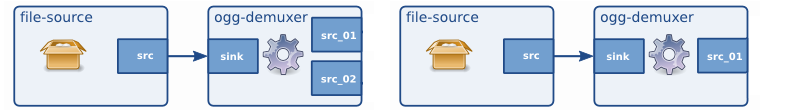
\includegraphics[width=150mm]{img/request-pads-demux.png}
  \caption{Dynamiczne pady elementu demuxera}
  \label{fig:requestPadsDemux}
\end{figure}
Ostatnia grupa, to gniazda, pojawiające się na żądanie użytkownika. Można wyobrazić sobie odwrotną sytuację do opisywanej w poprzednim akapicie. Użytkownik wstawia element muxera, który łączy kilka strumieni. W zależności od tego, ile strumieni użytkownik będzie chciał połączyć, tyle żądań o pad wejściowy będzie musiał zgłosić.

\end{document}. 
